%% LyX 2.4.0~beta5 created this file.  For more info, see https://www.lyx.org/.
%% Do not edit unless you really know what you are doing.
\documentclass[english,footrule]{foils}
\usepackage[T1]{fontenc}
\usepackage[latin9]{inputenc}
\pagestyle{foilheadings}
\setcounter{secnumdepth}{1}
\setcounter{tocdepth}{1}
\usepackage{color}
\usepackage{pifont}
\usepackage{amsmath}
\usepackage{amsthm}
\usepackage{amssymb}
\usepackage{graphicx}

\makeatletter

%%%%%%%%%%%%%%%%%%%%%%%%%%%%%% LyX specific LaTeX commands.
\newcommand{\noun}[1]{\textsc{#1}}
%% A simple dot to overcome graphicx limitations
\newcommand{\lyxdot}{.}


%%%%%%%%%%%%%%%%%%%%%%%%%%%%%% Textclass specific LaTeX commands.
\newenvironment{lyxcode}
	{\par\begin{list}{}{
		\setlength{\rightmargin}{\leftmargin}
		\setlength{\listparindent}{0pt}% needed for AMS classes
		\raggedright
		\setlength{\itemsep}{0pt}
		\setlength{\parsep}{0pt}
		\normalfont\ttfamily}%
	 \item[]}
	{\end{list}}

%%%%%%%%%%%%%%%%%%%%%%%%%%%%%% User specified LaTeX commands.
\newcommand{\argmin}{\operatornamewithlimits{argmin}}

\usepackage{xcolor}
\renewcommand{\labelitemi}{$\textcolor{blue}{\bullet}$}
\renewcommand{\labelitemii}{$\textcolor{teal}{\Rightarrow}$}
\renewcommand{\labelitemiii}{$\textcolor{red}{\rightarrow}$}
\renewcommand{\labelitemiv}{$\textcolor{brown}{\circ}$}

\newcommand{\T}{\mathrm{T}}  % transpose
\newcommand{\PP}{\mathrm{P}}  % probability
\newcommand{\dd}{\mathrm{d}} % integration dx
\newcommand{\ee}{\mathrm{e}} % exponential
\newcommand{\E}{\mathrm{E}} % expectation

%

\makeatother

\usepackage{babel}
\begin{document}

\MyLogo{Intro ML--Principal Component Analysis}
\title{Unsupervised Learning - Principal Compnent Analysis (PCA)}
\author{Mark Asch - IMU/VLP/CSU }
\date{2023}
\maketitle

\foilhead{Program}
\begin{enumerate}
\item Data Analysis

\begin{enumerate}
\item Introduction: the 4 identifiers of ``big data'' and ``data science''
\item Supervised learning methods: regression---advanced, k-NN, linear
classification methods, SVM, NN, decision trees. 
\item \textcolor{red}{Unsupervised learning methods}: \textcolor{red}{principal
component analysis}, k-means, clustering.
\end{enumerate}
\end{enumerate}

\foilhead{Introduction}
\begin{itemize}
\item \textcolor{magenta}{Supervised} learning: 

\begin{itemize}
\item we have $p$ characteristics $X_{1},X_{2},\ldots,X_{p}$ mesured on
$n$ observations 
\item one response $Y$ mesured on the same observations
\item objective: predict $Y$ using $X_{1},X_{2},\ldots,X_{p}$
\item methods: regression and classification
\end{itemize}
\item \textcolor{magenta}{Unsupervised} learning: 

\begin{itemize}
\item we \textcolor{magenta}{only }have $p$ characteristics $X_{1},X_{2},\ldots,X_{p}$
mesured on $n$ observations 
\item we want to make predictions, but we do not have an associated response
variable...
\item objective: \textcolor{magenta}{discover interesting effects} with
respect to the observations of $X_{1},X_{2},\ldots,X_{p}$ 

\begin{itemize}
\item Can we\textcolor{magenta}{{} visualize }or represent the data in a more
\textcolor{magenta}{informative} way? 
\item Can we \textcolor{magenta}{discover sub-groups or clusters} among
the variables or the observations? 
\end{itemize}
\end{itemize}
\end{itemize}

\foilhead{Warnings!}
\begin{itemize}
\item Unsupervised learning is more difficult, since it is subjective.
\end{itemize}
\begin{dinglist}{56}
\item Unsupervised learning is often part of an initial phase of \textcolor{magenta}{exploratory
data analysis} (EDA), where we compute elementary statistics and plot
basic histograms and boxplots-{}-{}-see Introductory lectures.
\item There are no universal \textcolor{magenta}{cross-validation} methods
for unsupervised learning. 
\item There is \textcolor{magenta}{no response variable} that can be used
to test our models.
\end{dinglist}
\begin{dinglist}{52}
\item However, there are a large number of application domains where unsupervised
learning is widely used.
\end{dinglist}

\foilhead{Introduction to PCA}
\begin{itemize}
\item PCA is a common approach for finding a \textcolor{magenta}{low dimensional}
ensemble of characteristics from a large set of variables.
\item It can be used for \textcolor{magenta}{dimension reduction} of an
$(n\times p)$ dimensional data matrix $X.$ Once this is done, 
\begin{itemize}
\item the direction of the \textcolor{magenta}{first principal component}
vector is that along which the observations vary the most, or it is
the direction that captures or explains the most variance in the observations. 
\item the principal components can form the basis for a \textcolor{magenta}{regression}---this
is principal component regression---see Regression lectures.
\end{itemize}
\item Principal component analysis is, by definition, the computation of
these principal components (directions) and their use for understanding
the data. 
\item PCA can also serve as a tool for visualizing the data, as an additional
technique of EDA.
\item A simple case is shown in the Figure below.
\end{itemize}
\begin{figure}
\begin{centering}
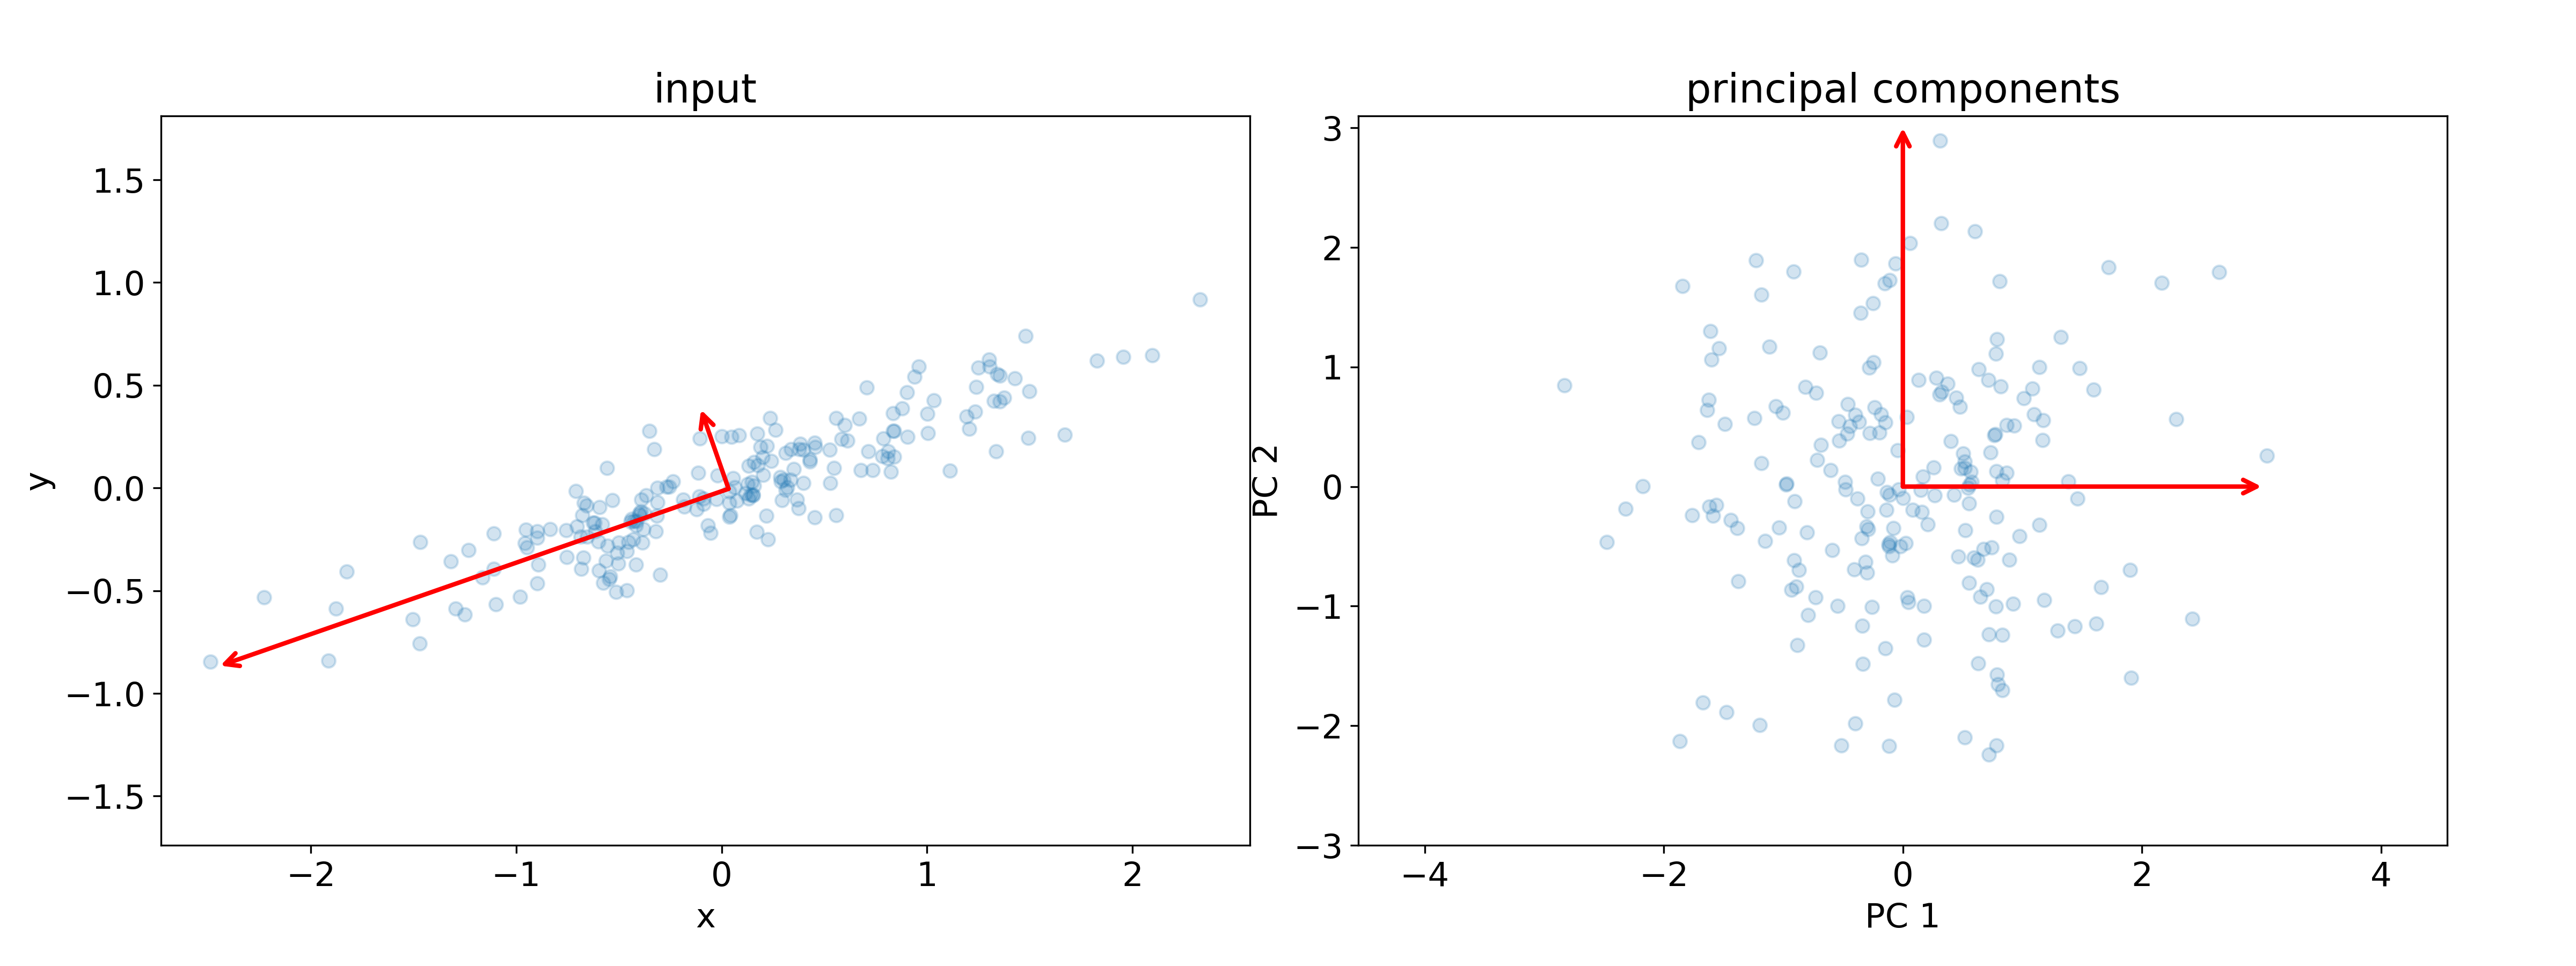
\includegraphics[width=1\paperwidth]{graphics/PCA2comp-rotation}
\par\end{centering}
\caption{PCA for a dataset with two features. In the left plot, we depict the
original data. The vectors represent the directions of the first and
the second principal components, and their lengths represent their
importance in terms of the amount of variance explained. The projection
of the data onto the two PCs is depicted in the right plot.}

\end{figure}


\foilhead{Theory}
\begin{itemize}
\item We want to visualize $n$ observations over a set of $p$ characteristics,
$X_{1},X_{2},\ldots,X_{p}.$ 
\begin{itemize}
\item We could do a\textcolor{magenta}{{} pairwise }scatterplot of the characteristics,
but the number of combinations, 
\[
\binom{p}{2}=p(p-1)/2,
\]
soon becomes very large. 
\end{itemize}
\item The PCA helps us to identify the smallest possible number of dimensions
(in the case where $p$ is large) that represent the largest possible
\textcolor{magenta}{proportion of the variation}. 
\item The \textcolor{magenta}{first principal component}, $Z_{1},$ is the
linear combination of the characteristics, 
\[
Z_{1}=\phi_{11}X_{1}+\phi_{21}X_{2}+\cdots+\phi_{p1}X_{p},
\]
with the largest variance, where
\begin{itemize}
\item $\sum_{j=1}^{p}\phi_{j1}^{2}=1$ (normalization), and 
\item $\phi_{11},\ldots,\phi_{p1}$ are the \textcolor{magenta}{loads} (coefficients).
\end{itemize}
\end{itemize}

\foilhead[-0.5in]{Computation of PCs}
\begin{itemize}
\item To compute the principal components, we suppose that 
\begin{itemize}
\item ${X}$ is a dataset of dimension $n\times p$ and that 
\item each variable in ${X}$ is centered (average equals zero), column-by-column. 
\end{itemize}
\item We seek a \textcolor{magenta}{linear combination} of the characteristics
of the form 
\[
z_{i1}=\phi_{11}x_{i1}+\phi_{21}x_{i2}+\cdots+\phi_{p1}x_{ip}
\]
that has a \textcolor{magenta}{maximal variance}, and whose coefficients
are \textcolor{magenta}{normalized}. 
\item Mathematically, we want to find 
\[
\max_{\phi_{11},\ldots,\phi_{p1}}\left\{ \frac{1}{n}\sum_{i=1}^{n}\left(\sum_{j=1}^{p}\phi_{j1}x_{ij}\right)^{2}\right\} ,
\]
such that 
\[
\sum_{j=1}^{p}\phi_{j1}^{2}=1.
\]
\item We remark the following:
\begin{itemize}
\item The quantity that we maximize is precisely the \textcolor{magenta}{empirical
variance} of $z.$ 
\item The optimization problem is solved by a decomposition into\textcolor{magenta}{{}
eigenvalues and eigenvectors }of the matrix ${X}^{\T}{X},$ 
\item The second principal component is the linear combination of maximal
variance that is non-correlated with the first principal component,
and thus orthogonal to it, and so on for the third, fourth, etc. 
\item Once the principal components have been computed, we can plot them
2-by-2 to obtain \textcolor{magenta}{low dimensional views }of the
data. This is the EDA aspect of PCA. 
\end{itemize}
\end{itemize}

\foilhead{PVE}
\begin{itemize}
\item The principal components represent the \textcolor{magenta}{proportion
of variance explained} (PVE). 
\begin{itemize}
\item Total variance for centered variables is, by definition, 
\[
V_{T}=\sum_{j=1}^{p}\textrm{Var}\left(X_{j}\right)=\sum_{j=1}^{p}\frac{1}{n}\sum_{i=1}^{n}x_{ij}^{2},
\]
\item Variance explained by the $m$-th principal component is 
\[
V_{m}=\frac{1}{n}\sum_{i=1}^{n}z_{im}^{2}=\frac{1}{n}\sum_{i=1}^{n}\left(\sum_{j=1}^{p}\phi_{jm}x_{ij}\right)^{2}.
\]
\item Then the proportion 
\[
\mathrm{PVE}=V_{m}/V_{T}
\]
gives us the variance explained.
\end{itemize}
\end{itemize}

\foilhead{How many PCs ?}

\index{scree plot!PCA} Please see the examples below.
\begin{itemize}
\item A matrix $\boldsymbol{X}$ of dimension $n\times p$ has $\min(n-1,p)$
distinct principal components 
\item The major question is: how many components one needs to adequately
describe the data. T
\item To decide this, we plot the PVE as a function of the principal component
number, in what is known as a ``\textcolor{magenta}{scree plot}.''
\begin{itemize}
\item The curve obtained will usually exhibit an ``\textcolor{magenta}{elbow},''
where the curvature changes sign. 
\item This point gives us the\textcolor{magenta}{{} optimal number} of principal
components to retain.
\end{itemize}
\end{itemize}
\begin{figure}
\begin{centering}
\noun{\includegraphics[scale=0.8]{\string"/Users/markasch/Dropbox/3Teaching/stat-ML/M2/03resources/ISLR/All Figures/Chapter10/10.4\string".pdf}}
\par\end{centering}
\caption{Scree Plot: left, the proportion of variance explained by each of
the 4 principal components; right, the cumulative proportion.}

\end{figure}


\foilhead[-0.5in]{Example: arrests in USA}
\begin{itemize}
\item the database \texttt{\textcolor{blue}{USArrests}} contains 50 states
and 4 variables: \texttt{\textcolor{blue}{Murder, Assault, UrbanPop,
Rape}}
\item the rows contain the 50 states in alphabetical order
\end{itemize}
\begin{lyxcode}
>~states~=row.names(USArrests~)~

>~states

{[}1{]}~\textquotedbl Alabama\textquotedbl ~~~~~~~~\textquotedbl Alaska\textquotedbl ~~~~~~~~~\textquotedbl Arizona\textquotedbl ~~~~~~~~~

{[}4{]}~\textquotedbl Arkansas\textquotedbl ~~~~~~~\textquotedbl California\textquotedbl ~~~~~\textquotedbl Colorado\textquotedbl ~~~~~~~~

{[}7{]}~\textquotedbl Connecticut\textquotedbl ~~~~\textquotedbl Delaware\textquotedbl ~~~~~~~\textquotedbl Florida\textquotedbl ~~~~~~~~

{[}10{]}~\textquotedbl Georgia\textquotedbl ~~~~~~~~\textquotedbl Hawaii\textquotedbl ~~~~~~~~~\textquotedbl Idaho\textquotedbl ~~~~~~~~~~

{[}13{]}~\textquotedbl Illinois\textquotedbl ~~~~~~~\textquotedbl Indiana\textquotedbl ~~~~~~~~\textquotedbl Iowa\textquotedbl ~~~~~~~~~~~

{[}16{]}~\textquotedbl Kansas\textquotedbl ~~~~~~~~~\textquotedbl Kentucky\textquotedbl ~~~~~~~\textquotedbl Louisiana\textquotedbl ~~~~~~

{[}19{]}~\textquotedbl Maine\textquotedbl ~~~~~~~~~~\textquotedbl Maryland\textquotedbl ~~~~~~~\textquotedbl Massachusetts\textquotedbl ~~

{[}22{]}~\textquotedbl Michigan\textquotedbl ~~~~~~~\textquotedbl Minnesota\textquotedbl ~~~~~~\textquotedbl Mississippi\textquotedbl ~~~~

{[}25{]}~\textquotedbl Missouri\textquotedbl ~~~~~~~\textquotedbl Montana\textquotedbl ~~~~~~~~\textquotedbl Nebraska\textquotedbl ~~~~~~~

...

{[}46{]}~\textquotedbl Virginia\textquotedbl ~~~~~~~\textquotedbl Washington\textquotedbl ~~~~~\textquotedbl West~Virginia\textquotedbl ~~

{[}49{]}~\textquotedbl Wisconsin\textquotedbl ~~~~~~\textquotedbl Wyoming\textquotedbl{}
\end{lyxcode}
\begin{itemize}
\item the columns contain the 4 variables
\end{itemize}
\begin{lyxcode}
>~names(USArrests)~

{[}1{]}~\textquotedbl Murder~\textquotedbl ~\textquotedbl Assault~\textquotedbl ~\textquotedbl UrbanPop~\textquotedbl ~\textquotedbl Rape\textquotedbl{}
\end{lyxcode}
\begin{itemize}
\item EDA: Let us examine the data. The averages and variances differ a
lot.
\end{itemize}
\begin{lyxcode}
>~apply(USArrests,~2,~mean)~

~Murder~Assault~UrbanPop~~Rape~

~~7.79~~~170.76~~~65.54~~~21.23

>~apply(USArrests,~2,~var)~

Murder~~Assault~~UrbanPop~~~Rape~

~~19.0~~~6945.2~~~~209.5~~~~~87.7
\end{lyxcode}
\begin{itemize}
\item Hence, we need to apply a scaling when using the function \texttt{\textcolor{blue}{prcomp()}}
that computes the principal components.
\end{itemize}
\begin{lyxcode}
>~pr.out=prcomp(USArrests,~scale=TRUE)
\end{lyxcode}
\begin{itemize}
\item The output contains a number of useful quantities
\end{itemize}
\begin{lyxcode}
>~names(pr.out)~

{[}1{]}~\textquotedbl sdev\textquotedbl ~\textquotedbl rotation~\textquotedbl ~\textquotedbl center~\textquotedbl ~\textquotedbl scale\textquotedbl ~\textquotedbl x\textquotedbl{}
\end{lyxcode}
\begin{itemize}
\item The variables \texttt{\textcolor{blue}{centre}} and \texttt{\textcolor{blue}{scale}}
correspond to the averages and standard deviations used in the scaling
\end{itemize}
\begin{lyxcode}
>~pr.out\$center~

Murder~~Assault~~UrbanPop~~Rape~

7.79~~~~170.76~~~~65.54~~~~21.23~

>~pr.out\$scale~

Murder~~Assault~~UrbanPop~~Rape~

4.36~~~~83.34~~~~~14.47~~~~~9.37
\end{lyxcode}
\begin{itemize}
\item The matrx \texttt{\textcolor{blue}{rotation}} provides the coefficients
of the 4 principal components 
\end{itemize}
\begin{lyxcode}
>~pr.out\$rotation~

~~~~~~~~~~~~PC1~~~~PC2~~~~PC3~~~~PC4~

Murder~~~-0.536~~0.418~-0.341~~0.649~

Assault~~-0.583~~0.188~-0.268~-0.743~

UrbanPop~-0.278~-0.873~-0.378~~0.134~

Rape~~~~~-0.543~-0.167~~0.818~~0.089
\end{lyxcode}
\begin{itemize}
\item To change the orientation and plot the projections of the original
variables d'origine on the first 2 principal directions/axes
\end{itemize}
\begin{lyxcode}
>~pr.out\$rotation=-pr.out\$rotation~

>~pr.out\$x=-pr.out\$x~

>~biplot(pr.out,~scale~=0)

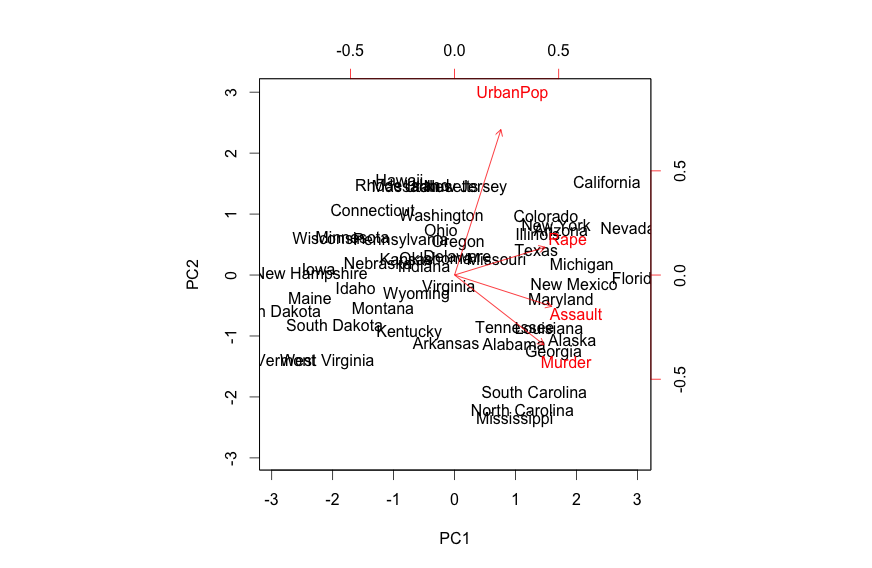
\includegraphics[scale=0.7]{graphics/pca-1}
\end{lyxcode}
\begin{itemize}
\item Compute the variance and the PVE
\end{itemize}
\begin{lyxcode}
>~pr.out\$sdev~

{[}1{]}~1.575~0.995~0.597~0.416

>~pr.var=pr.out\$sdev\textasciicircum 2~

>~pr.var~

{[}1{]}~2.480~0.990~0.357~0.173

>~pve=pr.var/sum(pr.var)~

>~pve~

{[}1{]}~0.6201~0.2474~0.0891~0.0434
\end{lyxcode}
\begin{itemize}
\item and plot them
\end{itemize}
\begin{lyxcode}
{\small >~par(mfrow=c(1,2))}{\small\par}

{\small >~plot(pve,xlab=\textquotedbl Principal~Component\textquotedbl ,ylab=\textquotedbl Proportion~}{\small\par}

{\small of~Variance~Explained\textquotedbl ,ylim=c(0,1),type=\textquoteright b\textquoteright )~}{\small\par}

{\small >~plot(cumsum(pve),xlab=\textquotedbl Principal~Component\textquotedbl ,ylab~=\textquotedbl Cumulative}{\small\par}

{\small Proportion~of~Variance~Explained\textquotedbl ,ylim=c(0,1),type=\textquoteright b\textquoteright )}{\small\par}
\end{lyxcode}
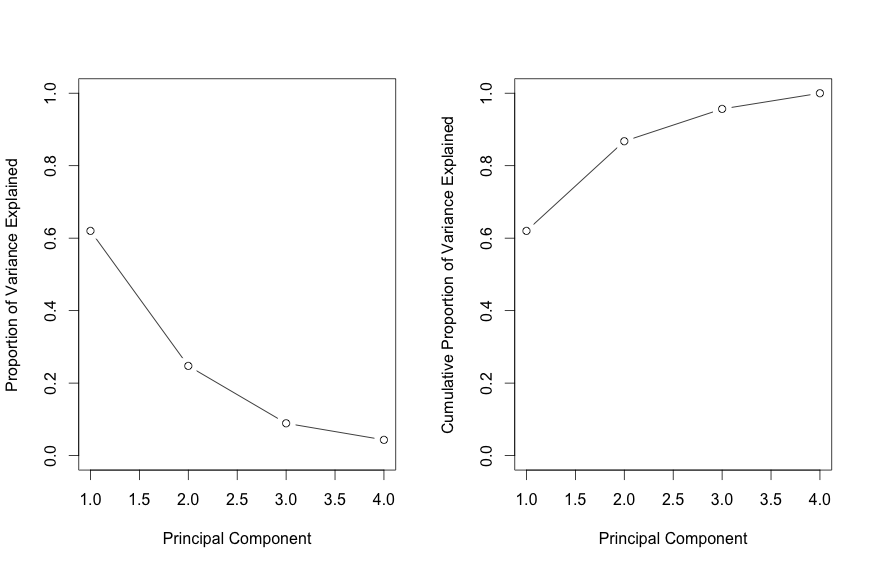
\includegraphics[width=0.6\textwidth]{graphics/pca-2}

\foilhead{Interpretation of PCA}
\begin{itemize}
\item After a PCA, the original \textcolor{magenta}{explnanatory variables}
are ``lost''
\item But, the \textcolor{magenta}{reduction of dimension} can elucidate
and facilitate the interpretaion and comprehension of all the data,
especially when the number of explanatory variables is (too) big
\item The interpretation always depends on the \textcolor{magenta}{context},
and should be done with the assistance of a domain expert:
\begin{itemize}
\item the first component is associated to all the violent crimes; 
\item the second component opposes assaults and murders with the population
(more violent crimes in the less populated states) ;
\item there is also a correlation between southern states and violent crimes,
with the exception of rape.
\end{itemize}
\end{itemize}

\foilhead{Examples}
\begin{enumerate}
\item The dataset \texttt{\textcolor{blue}{state.x77}} contains 8 explanatory
variables (4 more than \texttt{\textcolor{blue}{USArrests}}) and allows
to relate crimes with some socio-economical factors.
\item \texttt{\textcolor{blue}{PCA\_cars04}} is a very complete dataset
of cars from a consumer ascociation in the USA.
\item \texttt{\textcolor{blue}{PCA\_cancer}} contains breast cancer data.
We analyze it with \texttt{\textcolor{blue}{scikit-learn}}.
\end{enumerate}

\foilhead{References}
\begin{enumerate}
\item M. DeGroot, M. Schervish, \emph{Probability and Statistics}, Addison
Wesley, 2002.
\item Spiegel, Murray and Larry Stephens,\emph{ Schaum's Outline of Statistics,}
6th edition, McGraw Hill. 2017.
\item G. James, D. Witten, T. Hastie, R. Tibshirani. \emph{An Introduction
to Statistical Learning with Applications in R.} Springer. 2013.
\item T. Hastie, R. Tibshirani, J. Friedman. \emph{The Elements of Statistical
Learning}. Springer. 2009.
\item Rachel Schutt and Cathy O\textquoteright Neil. \emph{Doing Data Science.}
O'Reilly. 2014.
\end{enumerate}

\end{document}
